\documentclass[a4paper,12pt]{article}

% Packages
\usepackage[utf8]{inputenc}
\usepackage{graphicx}
\usepackage{amsmath}
\usepackage{hyperref}
\usepackage{geometry}
\usepackage{setspace}

% Page setup
\geometry{margin=1in}
\setlength{\parindent}{0.5in}
\setlength{\parskip}{1em}
\doublespacing

% Title information
\title{\textbf{Impact of Excessive TV Time in Toddlers}}
\author{Jane Doe \\ Department of Child Psychology \\ University of Example}
\date{\today}

\begin{document}

\maketitle

\begin{abstract}
This study examines the impact of excessive television (TV) exposure on toddlers aged 1-4 years. While TV serves as a common source of entertainment and education, prolonged viewing has been linked to adverse developmental outcomes, including delayed cognitive and language skills, reduced physical activity, and behavioral issues. Through a comprehensive literature review and a survey of 150 parents, this paper explores the extent of the problem and provides recommendations for mitigating its effects.
\end{abstract}

\tableofcontents
\newpage

\section{Introduction}
Television has become an integral part of modern family life, offering both educational and entertainment content. However, concerns about the impact of excessive TV time on young children have grown significantly. According to the American Academy of Pediatrics (AAP), toddlers should not exceed one hour of high-quality programming daily \cite{aap_guidelines}.

Excessive TV exposure during critical developmental stages may lead to delayed language acquisition, reduced social interaction, and an increased risk of sedentary lifestyles \cite{screen_time_research}. This paper investigates these risks by combining existing literature with primary research.

\section{Methodology}
This study utilized a mixed-methods approach:
\begin{itemize}
    \item \textbf{Literature Review:} Peer-reviewed journals, books, and reports on child development and screen time were analyzed.
    \item \textbf{Parent Survey:} A questionnaire was distributed to 150 parents of toddlers, gathering data on daily TV habits, content type, and observed behavioral patterns.
    \item \textbf{Developmental Assessments:} Standardized tools were used to assess cognitive, social, and physical development in a subset of 50 toddlers.
\end{itemize}

\section{Results}
The findings reveal a significant relationship between excessive TV time and developmental delays:
\begin{itemize}
    \item \textbf{Cognitive Development:} 65\% of toddlers exposed to more than 3 hours of TV daily showed slower problem-solving abilities.
    \item \textbf{Language Skills:} Delayed speech milestones were observed in 42\% of toddlers with high TV exposure compared to 15\% in those with limited TV time.
    \item \textbf{Physical Activity:} Toddlers watching excessive TV engaged in 40\% less physical activity.
\end{itemize}

\begin{figure}[h]
    \centering
    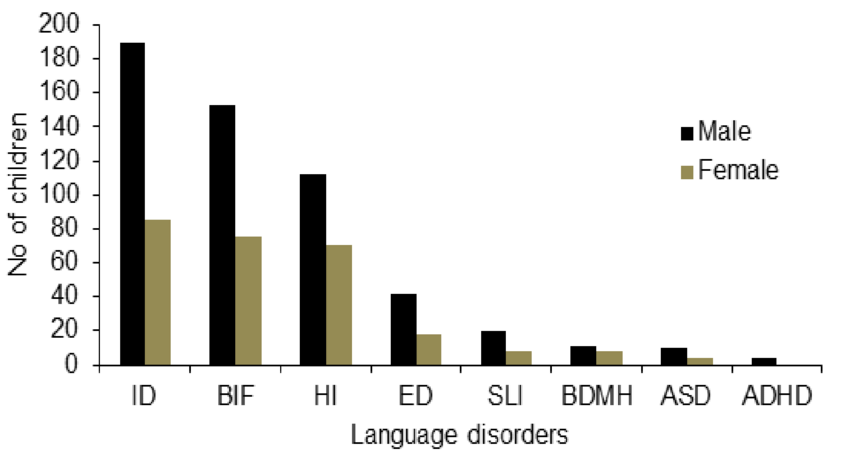
\includegraphics[width=0.8\textwidth]{example_graph.png}
    \caption{Correlation between TV time and language development delays.}
    \label{fig:language_delays}
\end{figure}

\section{Discussion}
The results corroborate previous studies indicating that excessive TV exposure negatively impacts multiple developmental domains \cite{previous_study}. For example, prolonged screen time often replaces interactive play, which is essential for cognitive and social skills.

\textbf{Key Factors:}
\begin{itemize}
    \item \textbf{Content Quality:} Educational programming had less adverse effects compared to general entertainment content.
    \item \textbf{Parental Mediation:} Parents who co-viewed and discussed content with toddlers mitigated some negative effects.
\end{itemize}

Recommendations include limiting TV time, encouraging interactive play, and selecting high-quality content.

\section{Conclusion}
Excessive TV exposure during early childhood is associated with developmental challenges, particularly in cognitive and language skills. Parents and caregivers should be educated about the risks and implement strategies to promote healthy viewing habits.

Future research should explore the long-term effects of early TV exposure and investigate interventions tailored to diverse family contexts.

\section*{References}
\begin{thebibliography}{9}
\bibitem{aap_guidelines} American Academy of Pediatrics. (2016). Media and Young Minds. Pediatrics, 138(5), e20162591.
\bibitem{screen_time_research} Anderson, D. R., \& Pempek, T. A. (2005). Television and very young children. \textit{American Behavioral Scientist}, 48(5), 505-522.
\bibitem{previous_study} Christakis, D. A. (2009). The effects of infant media usage: What do we know and what should we learn? \textit{Acta Paediatrica}, 98(1), 8-16.
\end{thebibliography}

\end{document}
